% document setup
\documentclass[12pt,a4paper]{article}
\usepackage[utf8]{inputenc}
\usepackage[ngerman]{babel}

% maths
\usepackage{amsfonts}
\usepackage{amssymb}
\usepackage{amsmath}

% utility
\usepackage[dvipsnames]{xcolor}
\usepackage{float}
\usepackage[colorlinks=false,linkbordercolor=red,urlbordercolor=red]{hyperref}
\usepackage{caption}
\usepackage[shortlabels]{enumitem}
\usepackage{tikz}

% useful commands
\newcommand{\qed}{\null\nobreak\hfill\square}

% title, author etc.
\title{Analysis I, Blatt 4}
\author{
    Gruppe 11\\
    Lorenz Bung (Matr.-Nr. 5113060)\\
    \href{mailto:lorenz.bung@students.uni-freiburg.de}{\texttt{lorenz.bung@students.uni-freiburg.de}}\\
    Charlotte Rothhaar (Matr.-Nr. 4315016)\\
    \href{mailto:charlotte.rothhaar97@gmail.com}{\texttt{charlotte.rothhaar97@gmail.com}}
}
\date{\today}

% begin document
\begin{document}

\maketitle


\section*{Aufgabe 13}

\begin{enumerate}[(i)]
    \item \textbf{Ansatz}: $a_n = \frac{f_{n+1}}{f_n} \Rightarrow f_{n+1} = f_n \cdot a_n$ und $a_{n-1} = \frac{f_n}{f_{n-1}} \Rightarrow f_n = f_{n-1} \cdot a_{n-1}$\\

    Damit erhalten wir
    $$a_{n+1} = \frac{f_{n+2}}{f_{n+1}} = \frac{a_{n+1} \cdot f_{n+1}}{a_n \cdot a_{n-1} \cdot f_{n-1}} = \frac{f_{n+2}}{a_n \cdot a_{n-1} \cdot \ldots \cdot a_0}$$

    \item Wir führen einen Beweis durch vollständige Induktion.\\

    \textbf{Induktionsbehauptung}: $1 \leq a_n \leq 2\ \forall n \in \mathbb{N}$.

    \textbf{Induktionsanfang ($n=0$)}: $1 \leq a_0 = \frac{f_1}{f_0} = \frac{1}{1} = 1 \leq 2$.

    \textbf{Induktionsschritt ($n \Rightarrow n+1$)}:
    \begin{align*}
    1 &\leq a_n = \frac{f_{n+1}}{f_n} \leq 2\\
    \Rightarrow 1 &\geq \frac{f_n}{f_{n+1}} \geq \frac{1}{2}\\
    \Rightarrow 2 &\geq 1 + \frac{f_n}{f_{n+1}} \geq \frac{3}{2}\\
    \Rightarrow 2 &\geq \frac{f_{n+1}}{f_{n+1}} + \frac{f_n}{f_{n+1}} = \frac{f_{n+1} + f_n}{f_{n+1}} \geq \frac{3}{2}\\
    \overset{\text{(Def. von } f_n\text{)}}{\Rightarrow} 2 &\geq \frac{f_{n+2}}{f_{n+1}} = \frac{f_{n+1+1}}{f_{n+1}} \geq \frac{3}{2}\\
    \Rightarrow 2 &\geq a_{n+1} \geq \frac{3}{2} > 1.
    \end{align*}

    Damit ist $1 \leq a_n \leq 2\ \forall n \in \mathbb{N}$.\\
    $\qed$

    \item \textbf{Behauptung}: $(a_{2n})_{n \in \mathbb{N}} := \frac{f_{2n+1}}{f_{2n}}$ ist monoton wachsend.\\

    \textbf{Beweis}: zu zeigen: $a_{2(n+1)} \geq a_{2n}$.\\
    Aus der Definition unserer Folge $(a_n)_n$ ergibt sich
    \begin{align*}
        a_{2(n+1)} = a_{2n+2} &\geq a_{2n}\\
        \frac{f_{2n+3}}{f_{2n+2}} = \frac{f_{2n+2} + f_{2n+1}}{f_{2n+1} + f_{2n}} &\geq \frac{f_{2n+1}}{f_{2n}} = \frac{2 f_{2n+1}}{f_{2n} + f_{2n+1}}\\
        \frac{f_{2n+2} - f_{2n+1}}{f_{2n+1} + f_{2n}} &\geq 0.
    \end{align*}
    Wegen $f_{2n+2} \geq f_{2n+1}$ ist der Nenner dieses Bruches immer positiv, und damit $\frac{f_{2n+2} - f_{2n+1}}{f_{2n+1} + f_{2n}} \geq 0$.\\
    Somit ist $(a_{2n})_n$ monoton wachsend.\\
    $\qed$

    \item \textbf{Behauptung}: Ja, $(a_n)_n$ konvergiert mit Grenzwert $a = \lim\limits_{n \to \infty} a_n = \Phi = \frac{1 + \sqrt{5}}{2}$.\\

    \textbf{Beweis}: Nach der Formel von Moivre-Binet ist
    $$f_n = \frac{1}{\sqrt{5}} \left(\Phi^n - \overline{\Phi}^n\right),\ \Phi = \frac{1 + \sqrt{5}}{2},\ \overline{\Phi} = \frac{1 - \sqrt{5}}{2}.$$
    Daher ist
    \begin{align*}
        a_n &= \frac{f_{n+1}}{f_n} = \frac{\frac{1}{\sqrt{5}}\left(\Phi^{n+1} - \overline{\Phi}^{n+1}\right)}{\frac{1}{\sqrt{5}}\left(\Phi^n - \overline{\Phi}^n\right)}\\
        &=\frac{\Phi^{n+1} - \overline{\Phi}^{n+1}}{\Phi^n - \overline{\Phi}^n}
        = \frac{\Phi^n \left(\Phi - \frac{\overline{\Phi}^{n+1}}{\Phi^n}\right)}{\Phi^n \left(1 - \frac{\overline{\Phi}^n}{\Phi^n}\right)}\\
        &= \frac{\Phi - \frac{\overline{\Phi}^{n+1}}{\Phi^n}}{1 - \frac{\overline{\Phi}^n}{\Phi^n}}
    \end{align*}
    und damit
    $$\lim\limits_{n \to \infty} a_n = \lim\limits_{n \to \infty} \frac{\Phi - \frac{\overline{\Phi}^{n+1}}{\Phi^n}}{1 - \frac{\overline{\Phi}^n}{\Phi^n}} = \frac{\Phi}{1} = \Phi.$$
    $\qed$
\end{enumerate}


\section*{Aufgabe 14}

\begin{enumerate}[(i)]
    \item Aufgrund der Eigenschaft $i^2 = -1$ ergeben sich vier Lösungen, die sich in Abhängigkeit von $n$ wiederholen:
    $$i^n = \left\lbrace\begin{matrix}
    1 & n = 0 \mod 4\\
    i & n = 1 \mod 4\\
    -1 & n = 2 \mod 4\\
    -i & n = 3 \mod 4
    \end{matrix}\right.,\ n \in \mathbb{N}$$

    \item Durch Erweitern des Bruches mit $\overline{3+2i} = 3-2i$ erhält man
    $$\frac{1+i}{3+2i} = \frac{(1+i)(3-2i)}{(3+2i)(3-2i)} = \frac{3+2-2i+3i}{9+4-6i+6i} = \frac{5+i}{13} = \frac{5}{13} + \frac{1}{13}i$$
    und damit die Werte $\frac{5}{13}$ für $a$ und $\frac{1}{13}$ für $b$.

    \item Die quadratische Gleichung $x^2 + px + q = 0,\ p,q \in \mathbb{R}$ hat höchstens zwei reelle Lösungen.

    \textbf{1. Fall}: Diskriminante $\left(\frac{p}{2}\right)^2 - q > 0 \Rightarrow$ 2 reelle Lösungen\\
    \textbf{2. Fall}: Diskriminante $\left(\frac{p}{2}\right)^2 - q = 0 \Rightarrow$ 1 reelle Lösung\\
    \textbf{3. Fall}: Diskriminante $\left(\frac{p}{2}\right)^2 - q < 0 \Rightarrow$ keine reelle Lösung.

    Im 3. Fall existieren zwei komplexe Lösungen für die Gleichung.

    \item Gleichungen vom Grad 3 haben in $\mathbb{C}$ 3 Lösungen.

    \textcolor{red}{\textbf{1. Lösung}}: $x^3 = e^{0 \cdot i} \Rightarrow x = e^{\frac{1}{3} \cdot 0 \cdot i} = 1$\\
    \textcolor{LimeGreen}{\textbf{2. Lösung}}: $x^3 = e^{2 \pi i} \Rightarrow x = e^{\frac{2}{3} \pi i}$ ($\frac{2}{3} \pi$ im Bogenmaß entspricht $120^\circ$)\\
    \textcolor{YellowOrange}{\textbf{3. Lösung}}: $x^3 = e^{4 \pi i} \Rightarrow x = e^{\frac{4}{3} \pi i}$ ($\frac{4}{3} \pi$ im Bogenmaß entspricht $240^\circ$)

    \begin{minipage}{\linewidth}
        \centering
        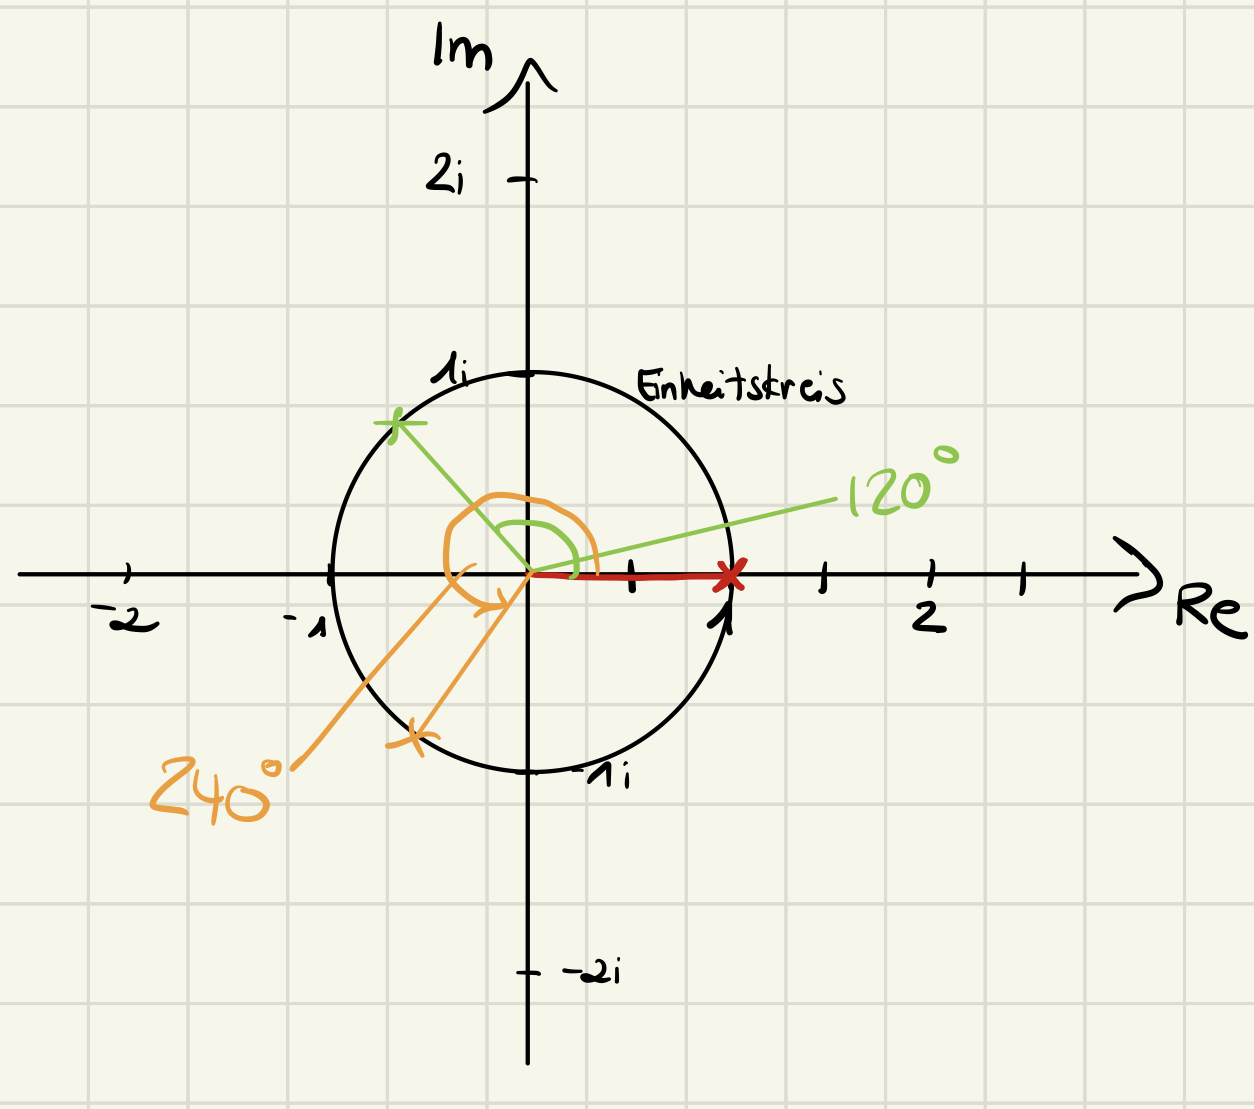
\includegraphics[width=0.5\textwidth]{a14iv.jpg}
        \captionof{figure}{}
        \label{fig:a14iv}
    \end{minipage}

    \item Ähnlich zu Aufgabenteil (i) wiederholen sich die Lösungen in Abhängigkeit von $n$:
    $$\left(\frac{1+i}{\sqrt{2}}\right)^n = \left\lbrace\begin{matrix}
    0 & n = 0 \mod 8\\
    \frac{1+i}{\sqrt{2}} & n = 1 \mod 8\\
    i & n = 2 \mod 8\\
    \frac{i-1}{\sqrt{2}} & n = 3 \mod 8\\
    -1 & n = 4 \mod 8\\
    \frac{-1-i}{\sqrt{2}} & n = 5 \mod 8\\
    -i & n = 6 \mod 8\\
    \frac{1-i}{\sqrt{2}} & n = 7 \mod 8
    \end{matrix}\right.,\ n \in \mathbb{N}.$$

    Diese lassen sich in einem Koordinatensystem im $\mathbb{R}^2$ darstellen, wobei die x-Achse den Realteil repräsentiert und die y-Achse den Imaginärteil:

    \begin{minipage}{\linewidth}
        \centering
        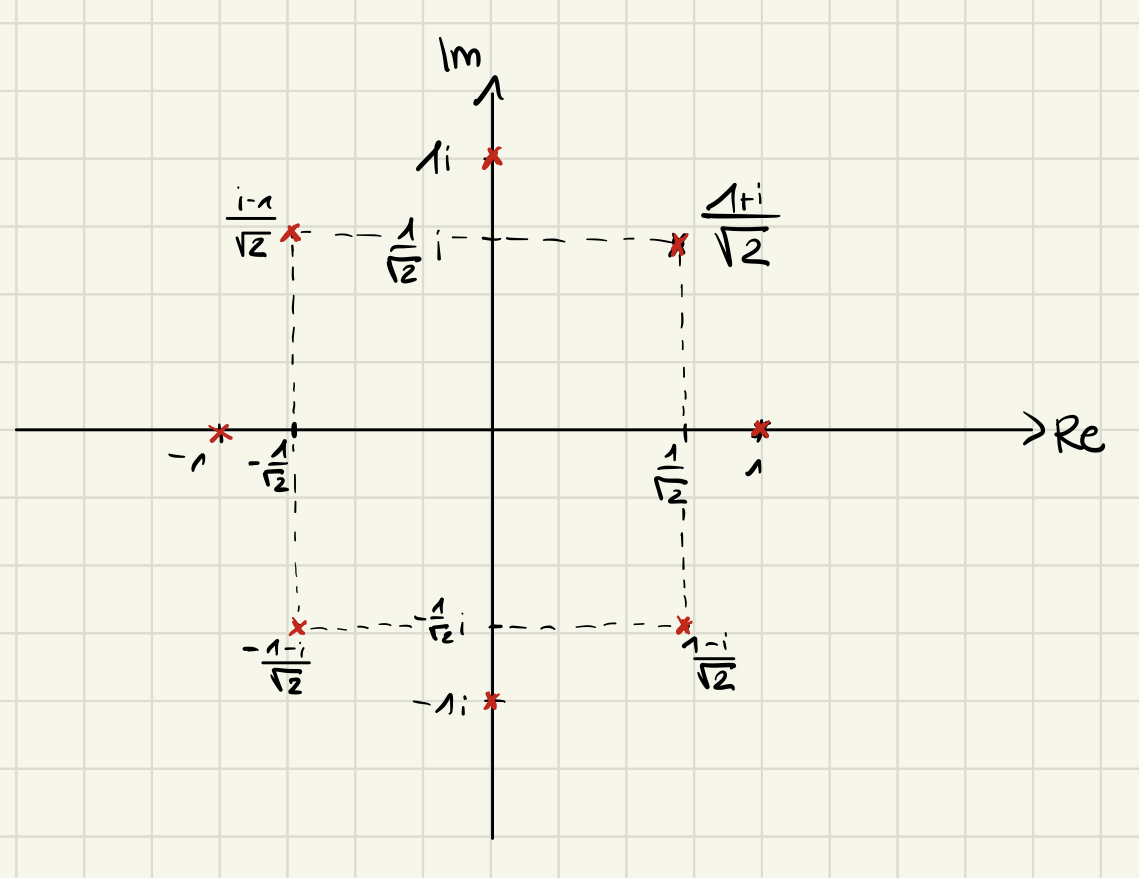
\includegraphics[width=0.5\textwidth]{a14v.jpg}
        \captionof{figure}{}
        \label{fig:a14v}
    \end{minipage}
\end{enumerate}


\section*{Aufgabe 15}

\begin{enumerate}[(i)]
    \item \textbf{zu zeigen}: $\sum\limits_{k=1}^\infty \left(a_k - a_{k-1}\right)$ ist konvergent $\Leftrightarrow \lim\limits_{n \to \infty} (a_n)_n$ existiert in $\mathbb{R}$.\\

    \textbf{Beweis}: ``$\Leftarrow$''\\
    Sei $(a_n)_n$ eine reelle Folge, die konvergiert.
    Dann ist $\lim\limits_{n \to \infty} a_n = \lim\limits_{n \to \infty} a_{n+1} = a$ und ferner $\lim\limits_{n \to \infty} a_n - \lim\limits_{n \to \infty} a_{n+1} = 0$.\\
    Daraus folgt für die Reihe, dass $(a_k - a_{k-1}) \to 0$ für $n \to \infty$.
    Wenn die Summanden der Reihe gegen 0 gehen, konvergiert die Reihe gegen einen Grenzwert $a$ mit
    \begin{align*}
        \sum\limits_{k=1}^n (a_k - a_{k-1}) &= (a_1 - a_0) + (a_2 - a_1) + \dots + (a_n - a_{n-1})\\
        &= (a_{n-1} - a_{n-2}) + (a_n - a_{n-1})\\
        &= (a_n - a_0)\\
        \sum\limits_{k=1}^\infty (a_k - a_{k-1}) &= a - a_0.
    \end{align*}

    \item Mithilfe von Partialbruchzerlegung ergibt sich
    $$\frac{1}{k(k+1)} = \frac{1+k-k}{k(k+1)} = \frac{1+k}{k(k+1)} - \frac{k}{k(k+1)} = \frac{1}{k} - \frac{1}{k+1}$$
    und damit $\sum\limits_{k=1}^\infty \frac{1}{k(k+1)} = \sum\limits_{k=1}^\infty \frac{1}{k} - \frac{1}{k+1}$.\\
    Aus Teilaufgabe (i) wissen wir, dass $\sum\limits_{k=1}^\infty a_k - a_{k+1} = a_n - a_0$ und damit analog $\sum\limits_{k=1}^\infty \frac{1}{a_k} - \frac{1}{a_{k+1}} = \frac{1}{a_k} - \frac{1}{a}$.\\
    Wegen $\frac{1}{a} = \frac{1}{\lim\limits_{n \to \infty} a_n} = 0$ ist somit
    $$\sum\limits_{k=2}^\infty \frac{1}{k(k+1)} = 1 - 0 = 1.$$\\

    $\frac{2}{k^2-1}$ hat Nullstellen bei $k_1 = 1$ und $k_2 = -1$.
    Auch hier kann man den Bruch nun mithilfe der Partialbruchzerlegung aufteilen in
    $$\frac{2}{k^2-1} = \frac{2}{(k+1)(k-1)} = \frac{\alpha}{k+1} + \frac{\beta}{k-1}.$$
    Es ergibt sich
    $$\frac{\alpha(k-1)+\beta(k+1)}{(k+1)(k-1)} \Rightarrow 2 = \alpha(k-1) + \beta(k+1)$$
    und somit $\beta = 1$ für $k = 1$ bzw. $\alpha = -1$ für $k=-1$.\\
    Insgesamt haben wir also
    $$\frac{2}{k^2-1} = \frac{1}{k-1} - \frac{1}{k+1}$$
    und damit
    $$\sum\limits_{k=2}^\infty \frac{2}{k^2-1} = \sum\limits_{k=2}^\infty \frac{1}{k-1} - \frac{1}{k+1}.$$
    Wegen $\lim\limits_{n \to \infty} \frac{1}{n+1} = 0$ folgt $\sum\limits_{k=2}^\infty \frac{2}{k^2-1} = 1 - 0 = 1.$\\
    $\qed$

    \item
\end{enumerate}


\section*{Aufgabe 16}

\begin{enumerate}[(i)]
    \item Da sich die Länge der Intervalle in jedem Schritt um $\frac{1}{3}$ verringert, lässt sich $s_n$ darstellen als
    \begin{align*}
    (s_n)_n &= \sum\limits_{i=0}^n M_i = M_0 + M_1 + M_2 + \dots + M_n\\
    &= 1 + \frac{2}{3} + \left(\frac{2}{3} \cdot \frac{2}{3}\right) + \dots + \left(\frac{2}{3}\right)^n = \sum\limits_{i=0}^n \left(\frac{2}{3}\right)^i.
    \end{align*}

    $(s_n)_n$ ist eine geometrische Reihe, da sie der Form $\sum\limits_{k=0}^\infty q^k$ entspricht.\\
    Aus $|q| = \left|\frac{2}{3}\right| = \frac{2}{3} < 1$ folgt, dass der Grenzwert die Form $\frac{q^m}{1-q}$ hat.\\
    Daher ist $\lim\limits_{n \to \infty} s_n = \frac{\left(\frac{2}{3}\right)^0}{1 - \frac{2}{3}} = \frac{1}{\frac{1}{3}} = 3$.
    Somit konvergiert die Reihe $(s_n)_n$ gegen den Grenzwert 3.\\
    $\qed$

    \item \begin{enumerate}[(a)]
        \item Da das mittlere Drittel der Dreiecksseite bei jedem Schritt durch ein doppelt so langes Stück ersetzt wird, wächst die Seitenlänge des Dreiecks pro Schritt um $\frac{4}{3}$.\\
        Für den $n$-ten Schritt ergibt sich so ein Umfang von $l_n = 3 \cdot \left(\frac{4}{3}\right)^n$.\\
        Es ist $\lim\limits_{n \to \infty} \frac{1}{l_n} = \lim\limits_{n \to \infty} \frac{1}{3 \cdot \left(\frac{4}{3}\right)^n} = \lim\limits_{n \to \infty} \left(\frac{3}{4}\right)^n = 0$, da es sich um eine geometrische Folge handelt und damit $\lim\limits_{n \to \infty} l_n = \lim\limits_{n \to \infty} \frac{1}{\frac{1}{l_n}} = \infty$.

        \item Zu Beginn hat das Dreieck einen Flächeninhalt von $A_0 = \frac{\sqrt{3}}{4}$, da es sich um ein gleichseitiges Dreieck handelt.
        Dieser Flächeninhalt wird nun im ersten Schritt um drei Dreiecke erweitert, im zweiten Schritt um $3 \cdot 4 = 12$ Dreiecke und im $n$-ten Schritt um $3 \cdot 4^n$ Dreiecke.\\
        Der Flächeninhalt der hinzugefügten Dreiecke beträgt dabei im ersten Schritt jeweils $\frac{\sqrt{3}}{4} \left(\frac{1}{3}\right)^2$, im zweiten Schritt dann nur noch $\frac{\sqrt{3}}{4} \left(\frac{1}{3} \cdot \frac{1}{3}\right)^2$ und im $n$-ten Schritt noch $\frac{\sqrt{3}}{4} \left(\frac{1}{9}\right)^n$.\\
        Damit ergibt sich pro Schritt ein Flächeninhalt von
        $$A_n - A_{n-1}= 3 \cdot 4^n \cdot \frac{\sqrt{3}}{4} \left(\frac{1}{9}\right)^n = 3 \frac{\sqrt{3}}{4} \left(\frac{4}{9}\right)^n.$$

        Der gesamte Flächeninhalt lässt sich nun also darstellen als
        $$A_n = A_0 + \sum\limits_{i=1}^n A_i - A_{i-1} = \frac{\sqrt{3}}{4} + \sum\limits_{i=1}^n 3 \frac{\sqrt{3}}{4} \left(\frac{4}{9}\right)^i.$$
        Dieser Flächeninhalt konvergiert für $n \to \infty$, denn
        \begin{align*}
        \sum\limits_{n=0}^\infty A_n =& \frac{\sqrt{3}}{4} + \sum\limits_{i=1}^\infty 3 \frac{\sqrt{3}}{4} \left(\frac{4}{9}\right)^i\\
        =& - 2 \frac{\sqrt{3}}{4} + \sum\limits_{n=0}^\infty \left(\frac{4}{9}\right)^i 3 \frac{\sqrt{3}}{4}
        \end{align*}
        und das ist bereits eine geometrische Reihe, welche konvergiert.
        Somit konvergiert auch die gesamte Summe.\\
        $\qed$
    \end{enumerate}
\end{enumerate}


% end document
\end{document}